% !TeX root = ../../tesi.tex

\subsection{Quantitative results}
The quantitative analysis of dough-ball volume was carried out on the three estimators introduced in Chapter~4: the depth-gap method, the rotated alpha-shape reconstruction, and the rotated convex-hull reconstruction. Tables~\ref{tab:volume_gap_stats}, \ref{tab:volume_rotated_alpha_stats}, and \ref{tab:volume_rotated_hull_stats} summarize the main descriptive statistics exported by the evaluation scripts.
For ground truth comparison, the expected volume interval was derived from the nominal weight of the dough balls(1.54 kg) and the typical density of the dough (approximately from 0.9 to 1.1 g/cm\textsuperscript{3}), resulting in an expected volume range of [1.38, 1.72] liters. The percentage of samples falling within this expected range was calculated for each estimator, providing a measure of how well the estimated volumes align with the nominal target interval. The depth-gap method showed a significantly lower percentage of samples within the expected range, as it was constantly understimating the volume.The rotated alpha-shape and convex-hull methods, demonstrated a much higher agreement with the nominal target interval. This suggests that the geometric reconstruction approaches (alpha-shape and convex-hull) provide more accurate volume estimates for the dough balls compared to the depth-gap method.
convex-hull estimator provides the highest percentage of samples inside the expected range, followed by the rotated alpha-shape estimator, while the depth-gap method yields a noticeably lower agreement with the nominal target interval.
convex-hull even though is built from the same point cloud as the alpha-shape, has a higher volume estimate, which is more in line with the expected range. This could be due to the fact that the convex-hull method captures the overall shape of the dough ball more effectively, while the alpha-shape method may be more sensitive to local variations and noise in the point cloud, leading to a slightly lower volume estimate. The depth-gap method, on the other hand, relies on a simpler approach that may not capture the full 3D structure of the dough ball, resulting in a significant underestimation of the volume.

\begin{table}[h]
    \centering
    \caption{Volume statistics obtained with the depth-gap estimator. Volumes are expressed in liters.}
    \label{tab:volume_gap_stats}
    \begin{tabular}{|l|r|}
        \hline
        Metric & Value \\
        \hline
        Original samples & 17766 \\
        Valid samples after filtering & 15902 \\
        Discarded outliers & 1864 \\
        Outlier interval & [0.500000, 2.600000] \\
        Mean volume & 1.153842 \\
        Median volume & 1.085705 \\
        Standard deviation & 0.313228 \\
        Minimum valid volume & 0.500858 \\
        Maximum valid volume & 2.599818 \\
        Expected interval & [1.380000, 1.720000] \\
        Derived interval from weight and density & [1.400000, 1.711111] \\
        Samples within expected range & 874 \\
        Samples within expected range (\%) & 5.50 \\
        \hline
    \end{tabular}
\end{table}

\begin{table}[h]
    \centering
    \caption{Volume statistics obtained with the rotated alpha-shape estimator. Volumes are expressed in liters.}
    \label{tab:volume_rotated_alpha_stats}
    \begin{tabular}{|l|r|}
        \hline
        Metric & Value \\
        \hline
        Original samples & 17739 \\
        Valid samples after filtering & 15185 \\
        Discarded outliers & 2554 \\
        Outlier interval & [0.700000, 2.600000] \\
        Mean volume & 1.523359 \\
        Median volume & 1.478649 \\
        Standard deviation & 0.286593 \\
        Minimum valid volume & 0.700107 \\
        Maximum valid volume & 2.599819 \\
        Expected interval & [1.380000, 1.720000] \\
        Derived interval from weight and density & [1.400000, 1.711111] \\
        Samples within expected range & 8746 \\
        Samples within expected range (\%) & 57.60 \\
        \hline
    \end{tabular}
\end{table}

\begin{table}[h]
    \centering
    \caption{Volume statistics obtained with the rotated convex-hull estimator. Volumes are expressed in liters.}
    \label{tab:volume_rotated_hull_stats}
    \begin{tabular}{|l|r|}
        \hline
        Metric & Value \\
        \hline
        Original samples & 17740 \\
        Valid samples after filtering & 15261 \\
        Discarded outliers & 2479 \\
        Outlier interval & [0.800000, 2.600000] \\
        Mean volume & 1.581481 \\
        Median volume & 1.544832 \\
        Standard deviation & 0.260279 \\
        Minimum valid volume & 0.800663 \\
        Maximum valid volume & 2.599514 \\
        Expected interval & [1.380000, 1.720000] \\
        Derived interval from weight and density & [1.400000, 1.711111] \\
        Samples within expected range & 10338 \\
        Samples within expected range (\%) & 67.74 \\
        \hline
    \end{tabular}
\end{table}
\newpage
The rotated convex-hull estimator provides the highest percentage of samples inside the expected range, followed by the rotated alpha-shape estimator, while the depth-gap method yields a noticeably lower agreement with the nominal target interval.

\begin{figure}[h]
    \centering
    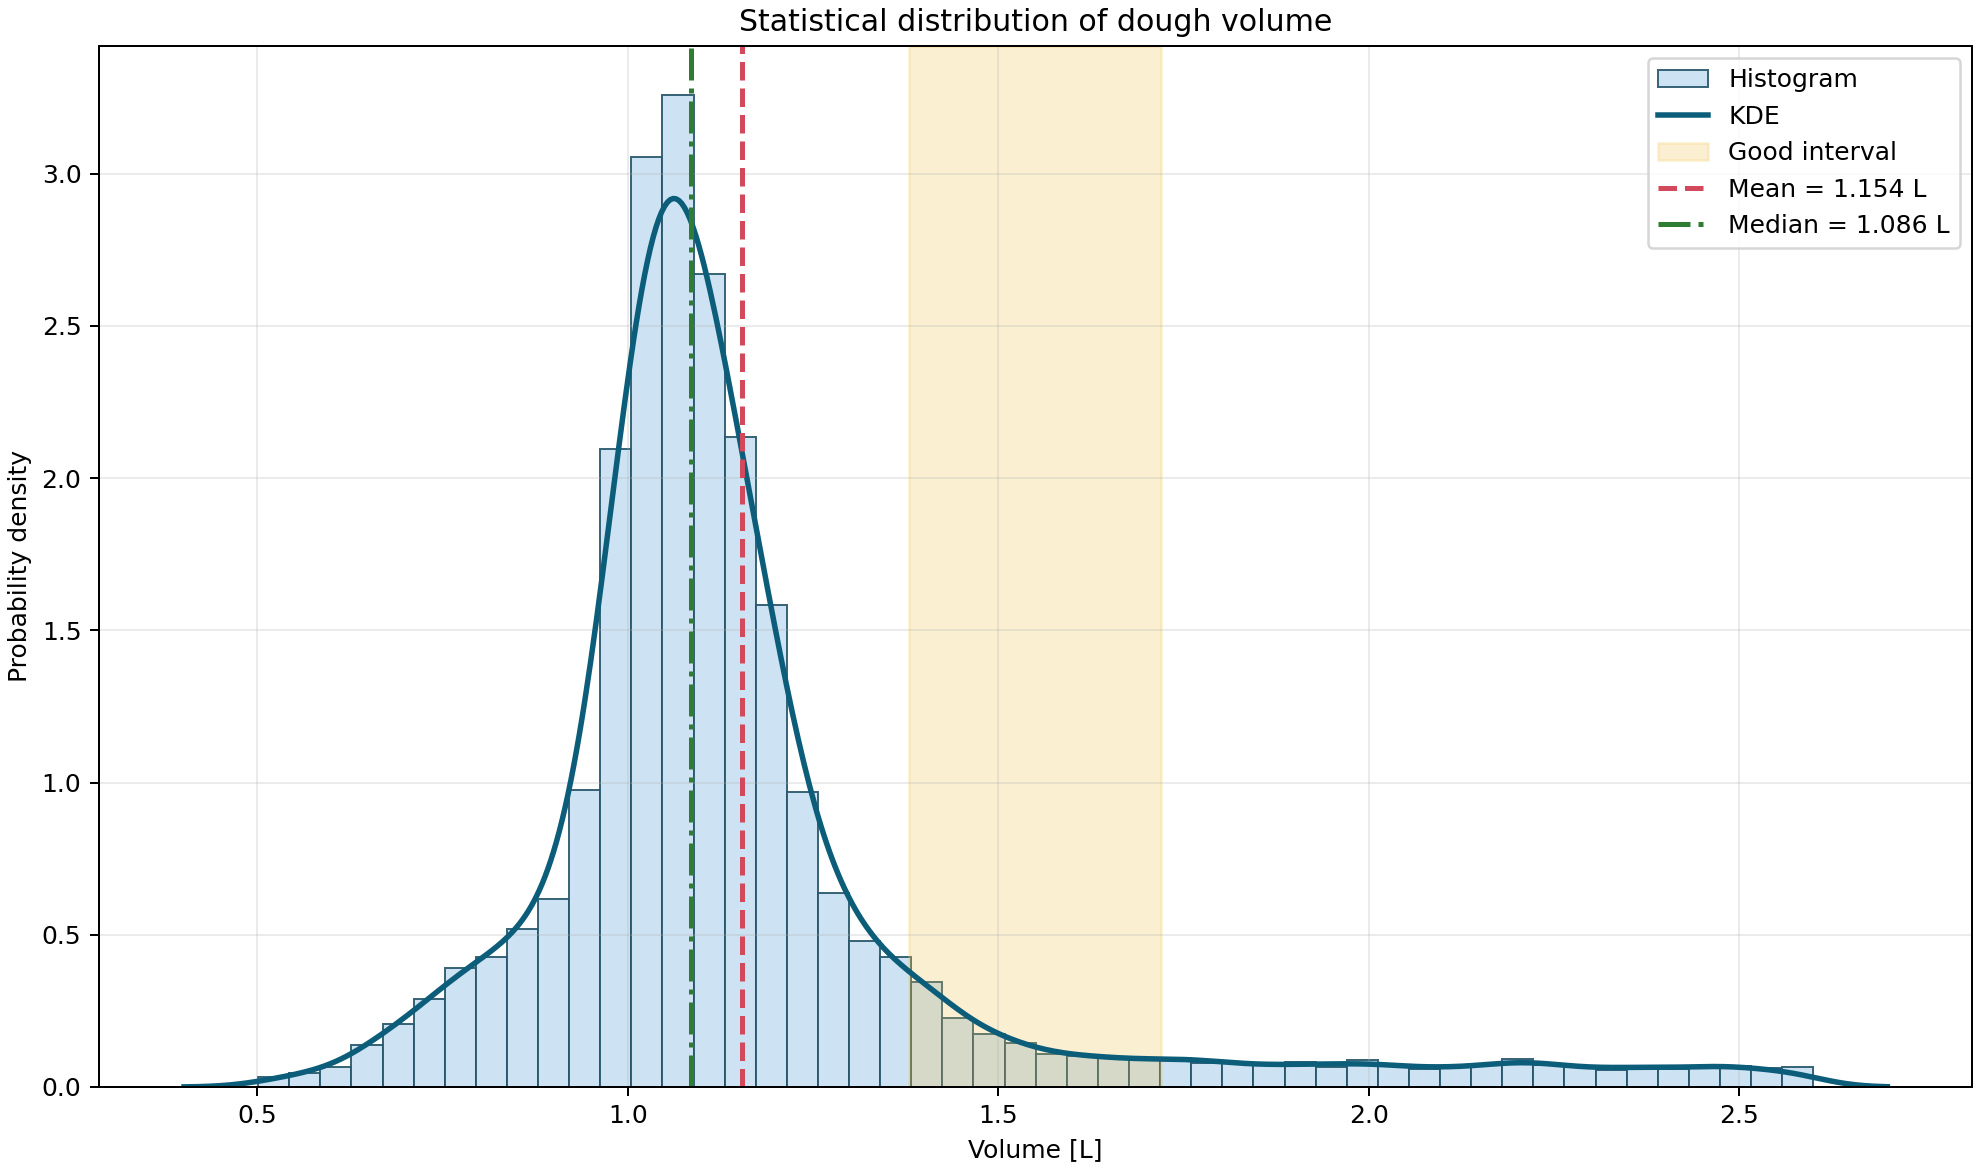
\includegraphics[width=\textwidth]{images/RESULTS/Volume/volume_distribution_gap.png}
    \caption{Volume distribution obtained with the depth-gap estimator.}
    \label{fig:volume_gap}
\end{figure}

\begin{figure}[h]
    \centering
    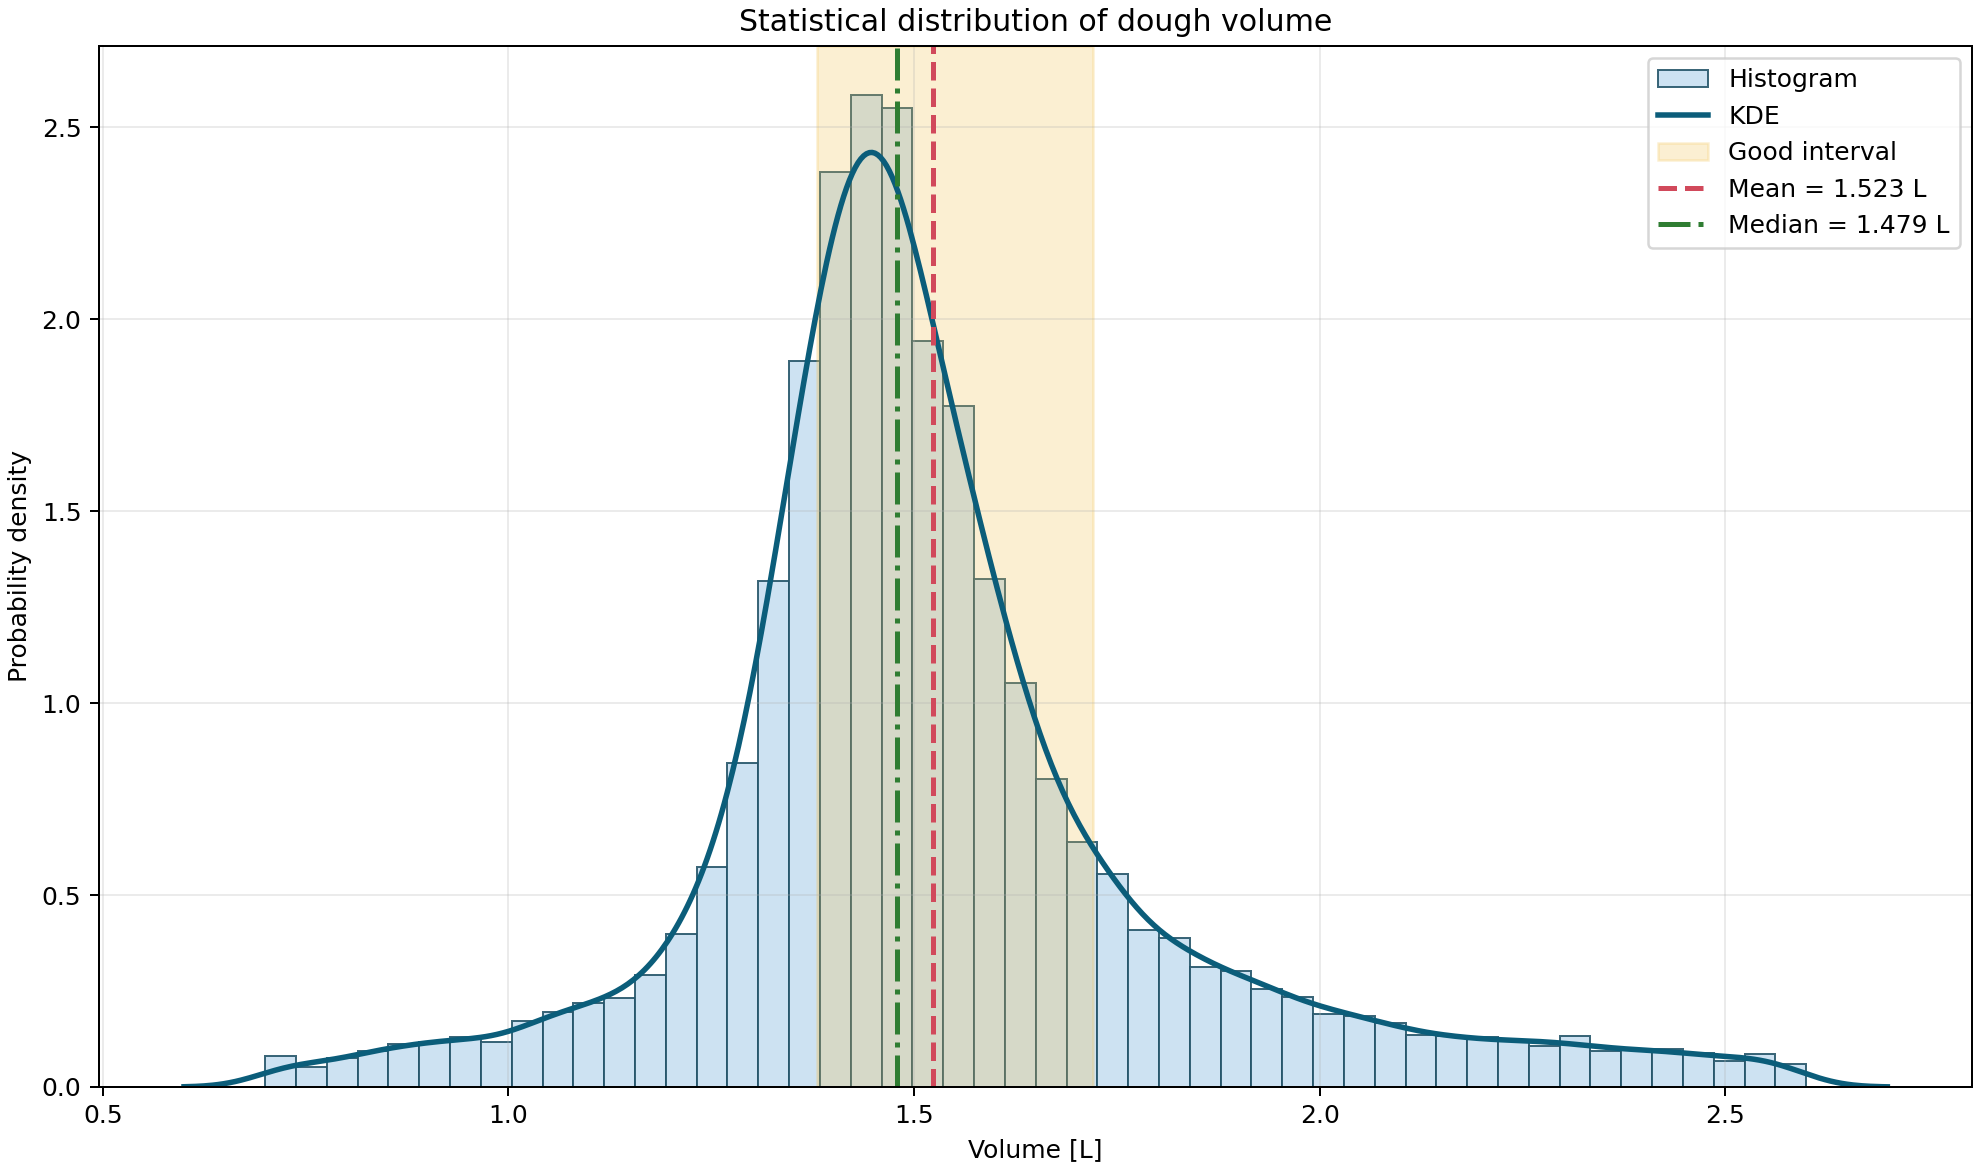
\includegraphics[width=\textwidth]{images/RESULTS/Volume/volume_distribution_rotated_alpha.png}
    \caption{Volume distribution obtained with the rotated alpha-shape estimator.}
    \label{fig:volume_rotated_alpha}
\end{figure}

\begin{figure}[h]
    \centering
    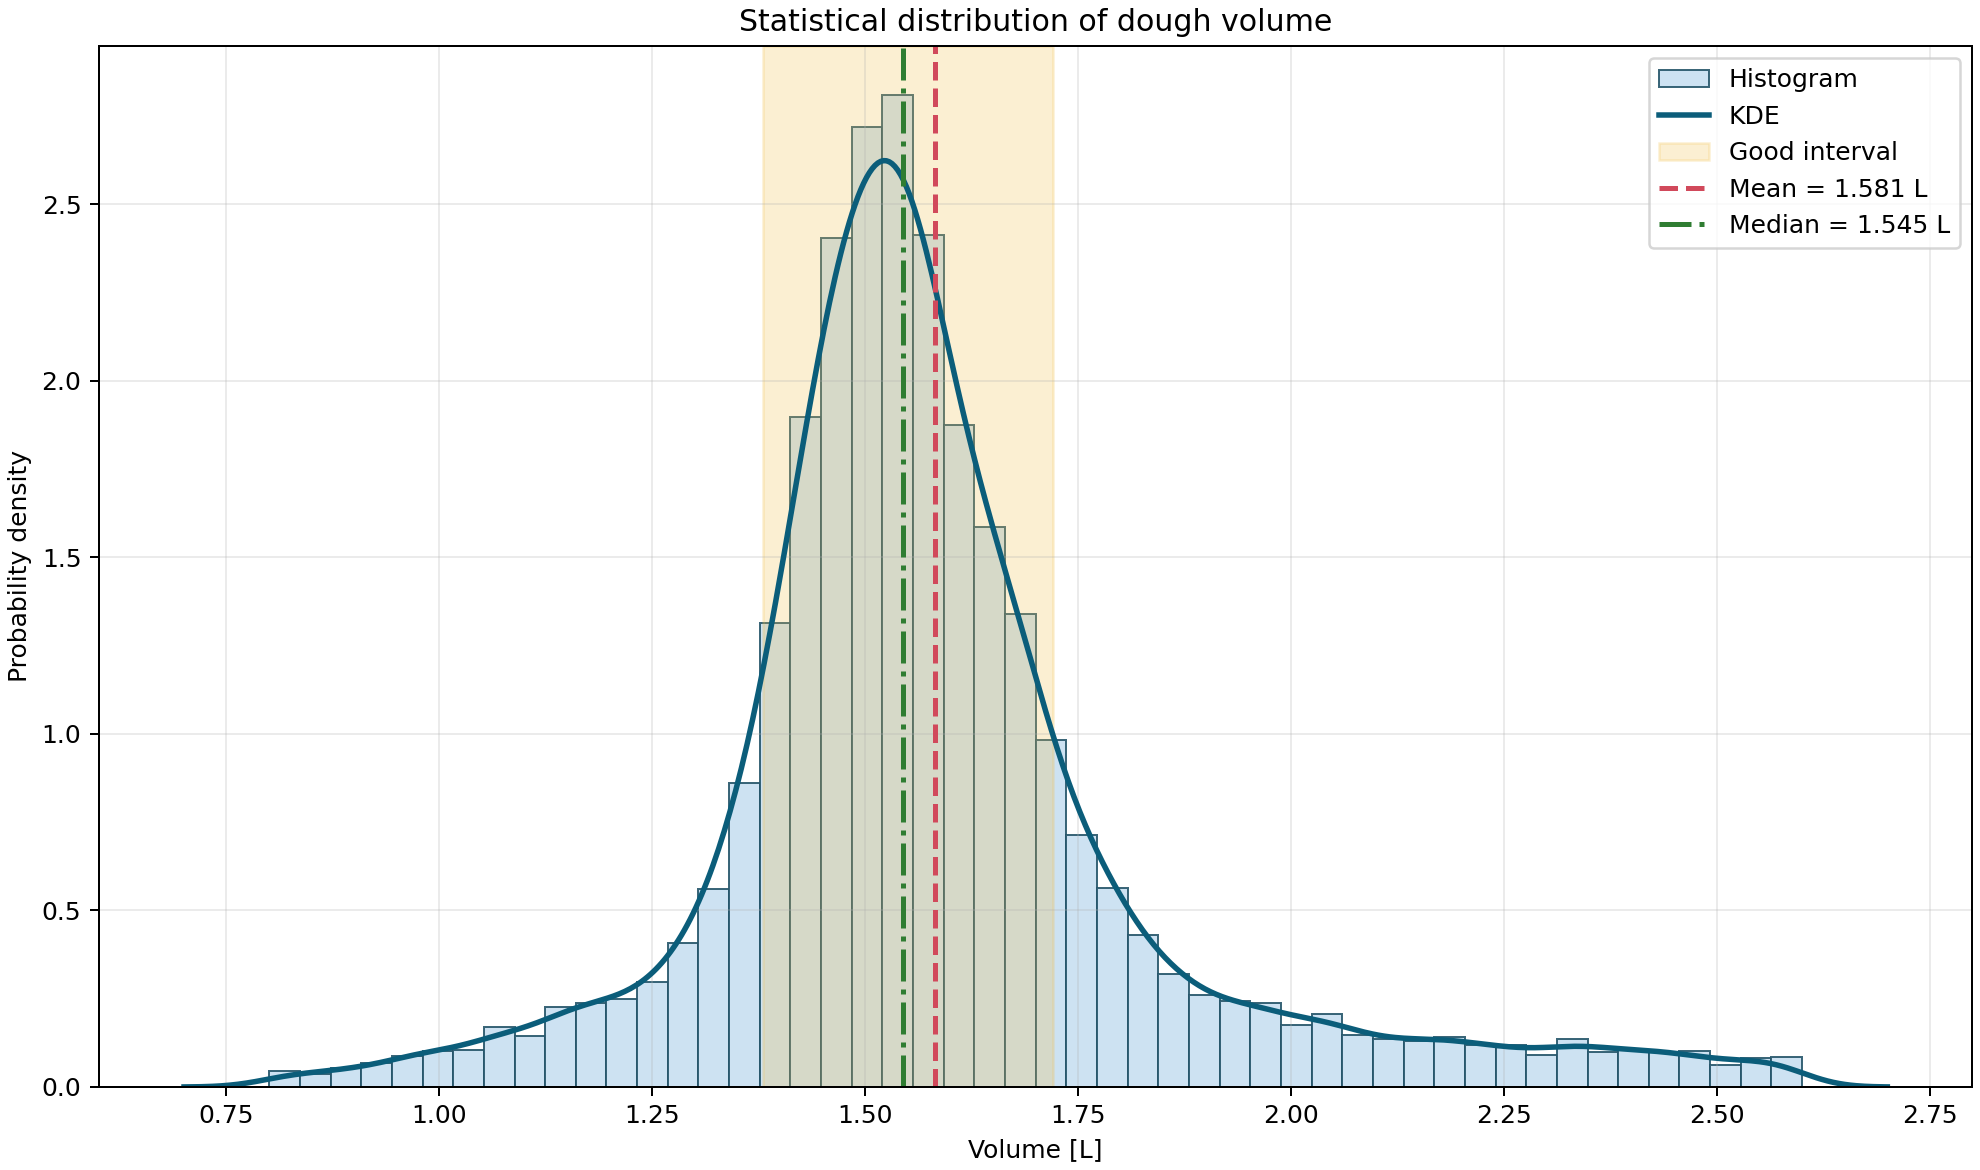
\includegraphics[width=\textwidth]{images/RESULTS/Volume/volume_distribution_rotated_hull.png}
    \caption{Volume distribution obtained with the rotated convex-hull estimator.}
    \label{fig:volume_rotated_hull}
\end{figure}

\begin{figure}[h]
    \centering
    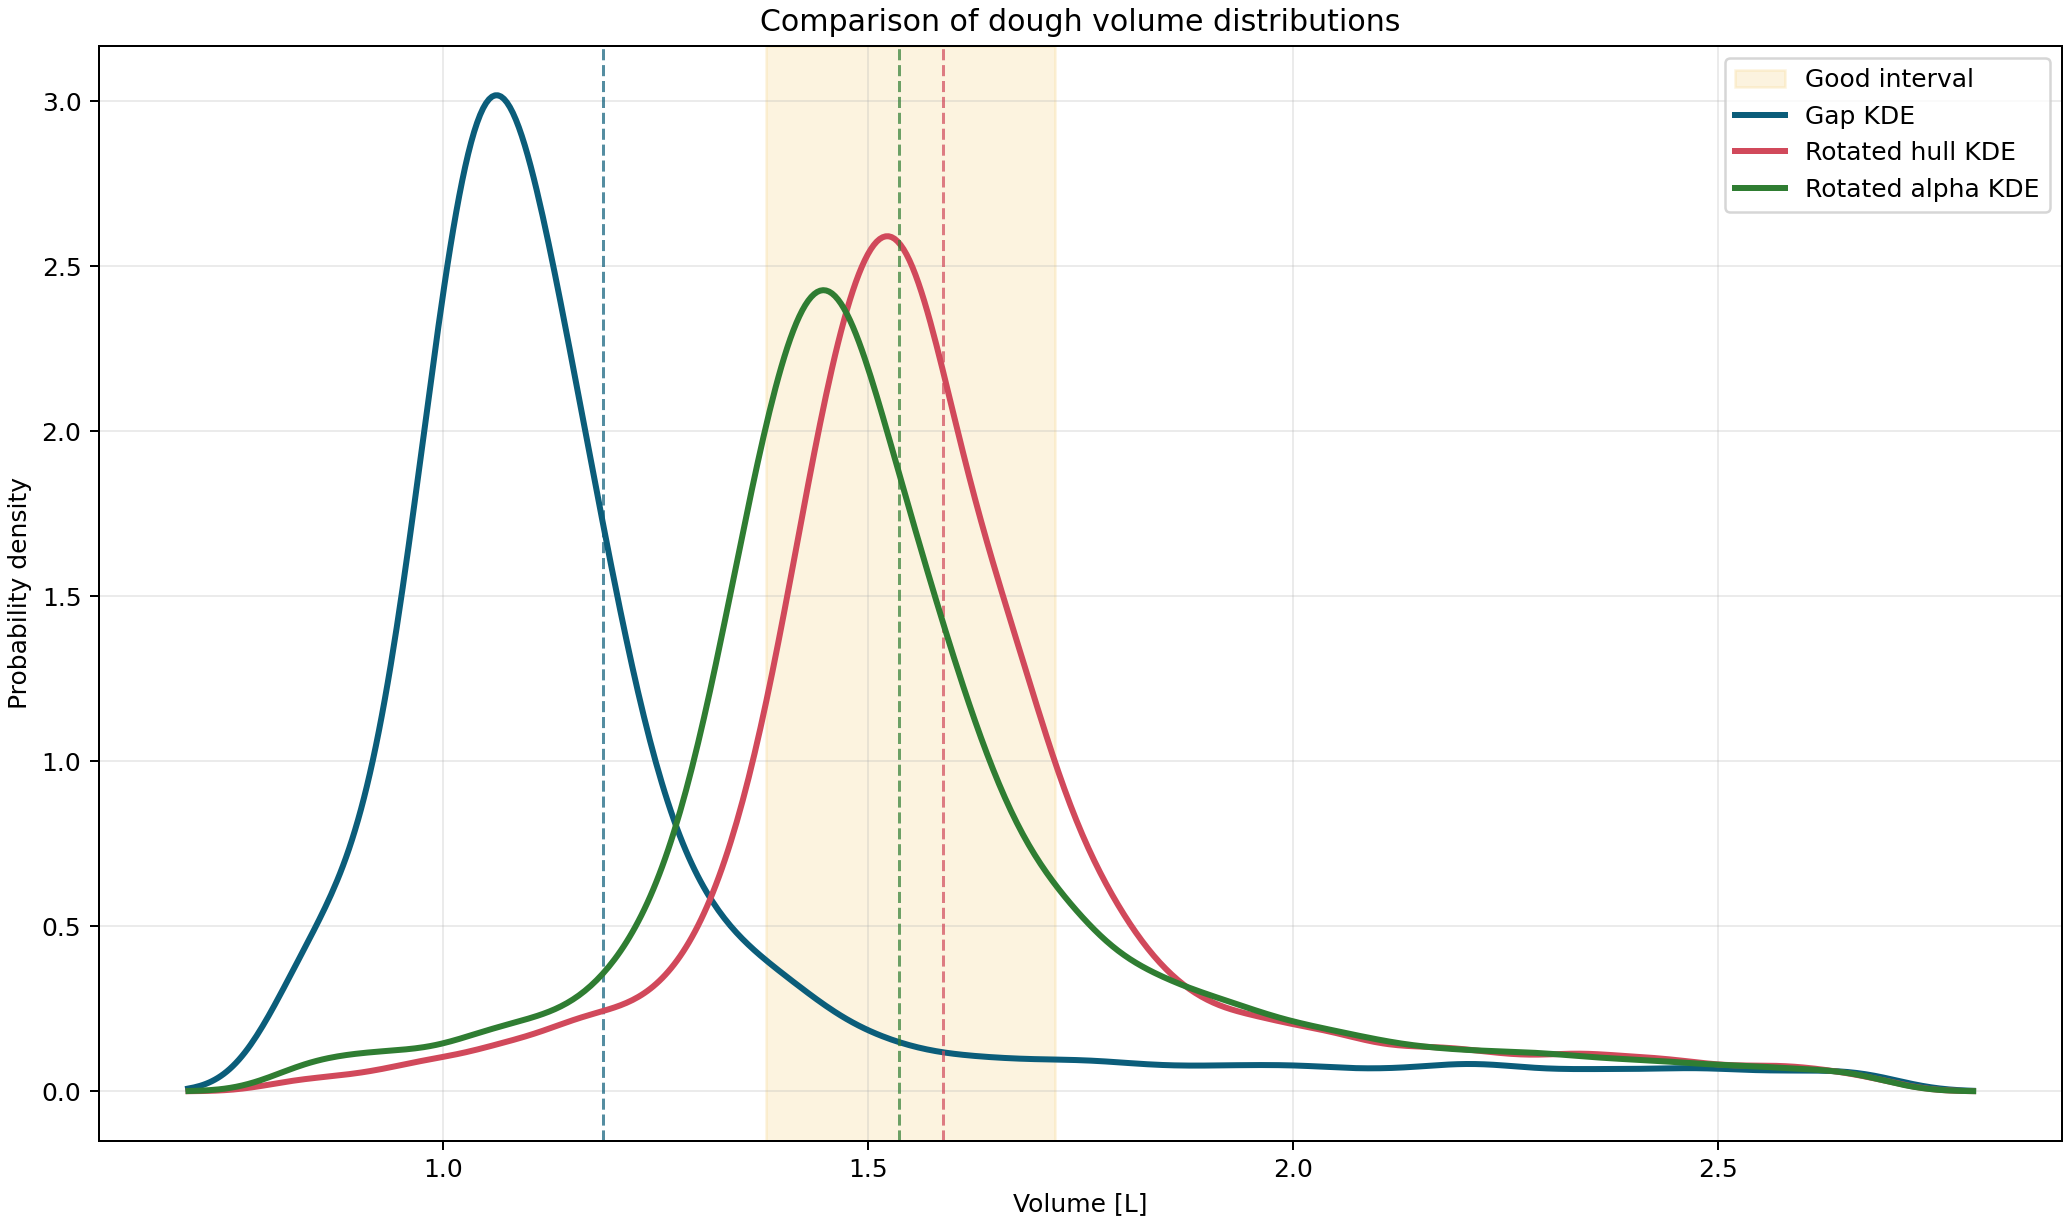
\includegraphics[width=\textwidth]{images/RESULTS/Volume/volume_distribution_comparison.png}
    \caption{Comparison of the volume distributions obtained with the three estimators.}
    \label{fig:volume_comparison}
\end{figure}

\subsection{Qualitative results}
\begin{figure}[h]
    \centering
    
\includegraphics[width=\textwidth]{"images/Useful-photos/Screenshots/Screenshot from 2026-04-05 12-40-59.png"}
    \caption{Example of qualitative results for dough-ball volume estimation at Site~1. The figure shows the original RGB image with detected dough balls, the corresponding depth map, and the 3D point cloud representation used for volumetric analysis. The estimated volume for each dough ball is displayed alongside the visualizations.}
    \label{fig:3D_volume_rendering}
\end{figure}
